\chapter{Statistics - Basic}

\textit{In any chapter in this book, especially in this chapter, I will assume (1) you have really basic knowledge on statistics, e.g., what ``Gaussian'', ``probability'', ``standard normal distribution'' means and/or (2) you know how to use Google so that you can find concepts which you don't know.}

Let's start with a question. 
\begin{ex}
  For the \textbf{same star}, consider the following three scenarios:
  \begin{itemize}
    \item Case A: Researcher 1 says $ m_1 =  \m{14.0} \pm \m{0.1} $; Researcher 2 says $ m_2 = \m{15.0} \pm \m{1.0} $.
    \item Case B: Researcher 1 says $ m_1 =  \m{14.0} \pm \m{0.1} $; Researcher 2 says $ m_2 = \m{15.0} \pm \m{0.3} $.
    \item Case C: Researcher 1 says $ m_1 =  \m{14.0} \pm \m{0.1} $; Researcher 2 says $ m_2 = \m{15.0} \pm \m{0.1} $.
  \end{itemize}
  For each of the three cases: Are the two studies coincide? If so, with how much confidence would you say so? Wait, but what does that ``$ \pm $'' sign means in rigorous mathematical sense?
\end{ex}

Some of the previous course takers answered that they coincide, because the ``3-sigma rule'' says, e.g., for case A, $ m_1 = \m{14.0} \pm \m{0.3} $ \& $ m_2 = \m{15.0} \pm \m{3.0} $ overlaps with each other. Crudely speaking, this makes sense, but it is of course not the ``publication level'' reasoning.

To give you the answer: It is an ill-defined question. The answer can change based on the number of observations each reasercher used for the determination of the magnitude. If we assume that number is 5 for both researchers, for example, we can give some meaningful answers: We \textit{cannot reject} $ m_1 = m_2 $ for case A \& B with 90 \% confidence, and we \textit{can reject} $ m_1 = m_2 $ for case C with 90 \% confidence. Depending on the confidence level, the answer may change. Also the expression that \textit{can/cannot reject} is very important! You shouldn't say you \textit{accept $ m_1 = m_2 $}. Let me explain why throughout this chapter.


\section{The $ n $-$ \sigma $} \label{sec: n-sigma notation}
Maybe you are familiar of the 1-$ \sigma $, 2-$ \sigma $, and 3-$ \sigma $ words (cf. \cref{fig:nsigmawiki}). For example, mean $ \pm 1$-$ \sigma $ contains $ 68.27\cdots \% $ of the total area. Similarly 3-$ \sigma $ conatains $ 99.73\cdots \% $ of it, so it is very unlikely to get a sample outside of the mean $ \pm 3 $-$ \sigma $. 

\begin{figure}[ht!]
  \centering
  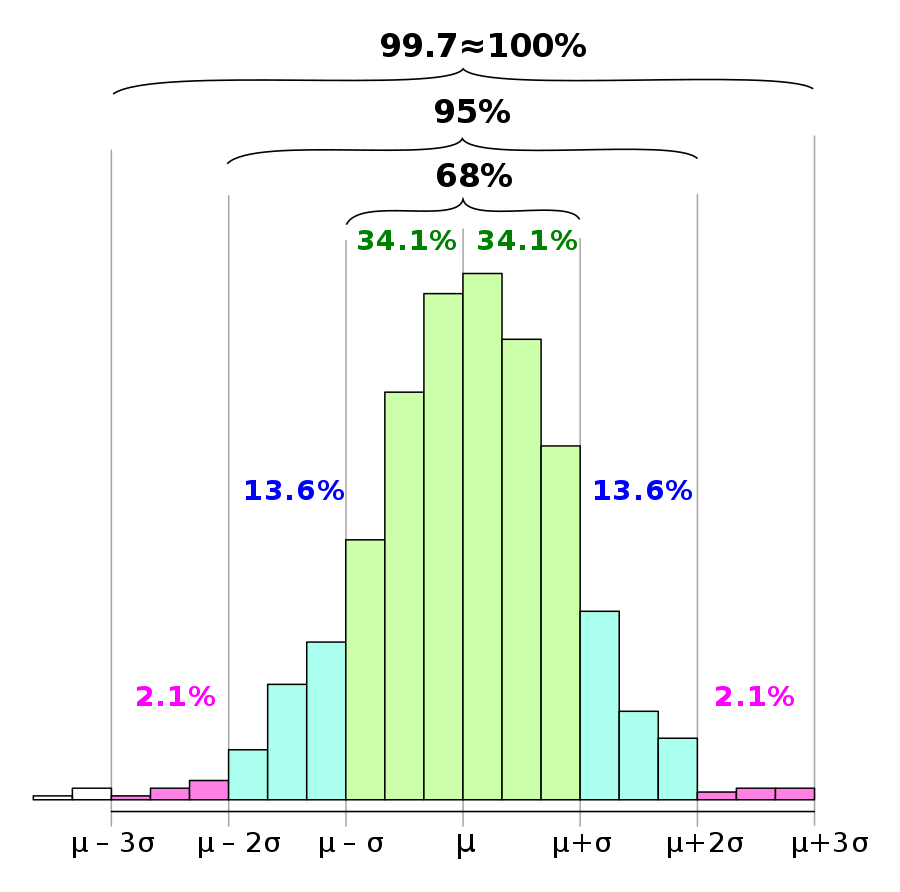
\includegraphics[width=0.5\linewidth]{figs/nsigma_wiki}
  \caption{A test sampling from Gaussian (normal) distribution (from Wikimedia).}
  \label{fig:nsigmawiki}
\end{figure}

In this sense, the ``$ n $-$ \sigma $'' is defined as the $ x $-axis value which gives the integrated area of certain value. More precisely, we have to call this confidence interval (CI):

\begin{defn}[$ n $-$ \sigma $ Confidence Interval; CI]
  1-$ \sigma $ CI is the integrated area is $ 0.6827\cdots $ of the total area. Similarly, 2-$ \sigma $ CI is that with $ 0.9545\cdots $, 3-$ \sigma $ CI is that with $ 0.9973\cdots $, etc. 
\end{defn}

Mathematically it is more correct to call, e.g., 1-$ \sigma $ CI as the $ 68.27\cdots \% $ CI. We also define the significance level $ \alpha $ as 100\% minus this percentage, i.e., the 1-$ \sigma $ CI is of significance level $ \alpha = 1 - 0.6827\cdots = 0.3173\cdots $:
\begin{equation}
  \text{1-}\sigma \text{ CI}
  \quad \equiv \quad 
  68.27\cdots \% \text{ CI}
  \quad \equiv \quad 
  \text{CI of significance level } 0.3173 \cdots ~.
\end{equation}
In natural sciences we often use $ n $-$ \sigma $ CI, but in mathematics and other branches of sciences and engineering, the 90 \%, 95 \%, and 99 \% CIs, i.e., CIs with significance level $ \alpha = 0.10,\, 0.05,$ and $ 0.01 $ are used more often.

Because when we say ``$ n $-$ \sigma $'', we are just omitting the term ``CI'' at the end of it, this is not $ n $ times the standard deviation ($ \sigma $): What we mean by ``$ n $-$ \sigma $'' is actually ``$ n $-$ \sigma $ CI'' and is \textit{not necessarily} $ n \times \sigma $. 

They are the same for, e.g., Gaussian distribution. For Gaussian (normal) distribution, which is a distribution that appears very often in natural sciences, such a 2-$ \sigma $ is nothing but 2 times the standard deviation ($ \sigma $). For almost all of the distributions other than Gaussian, this is not the case.



\section{The Meaning of $ \pm $ Sign}
Simple answer: The $ \pm $ sign means the 1-$ \sigma $ confidence interval (CI). It is also simply called as the ``error-bar''. 

Honestly speaking, the $ \pm $ sign, i.e., the 1-$ \sigma $ CI, does \textit{not} fully describe the uncertainty. The best way to show or describe the uncertainty is to show a graph of probability distribution function (pdf or p.d.f.) as in \cref{fig:figposterior01}. In many but not all publications or books, people do not show this, because (1) the distribution is very similar to Gaussian or certain widely known distribution and it is clearly written in the text or assumed as all the readers know that, (2) detailed calculation is not of interest and/or does not affect the final result, (3) the writer is lazy. 

\begin{figure}[ht!]
\centering
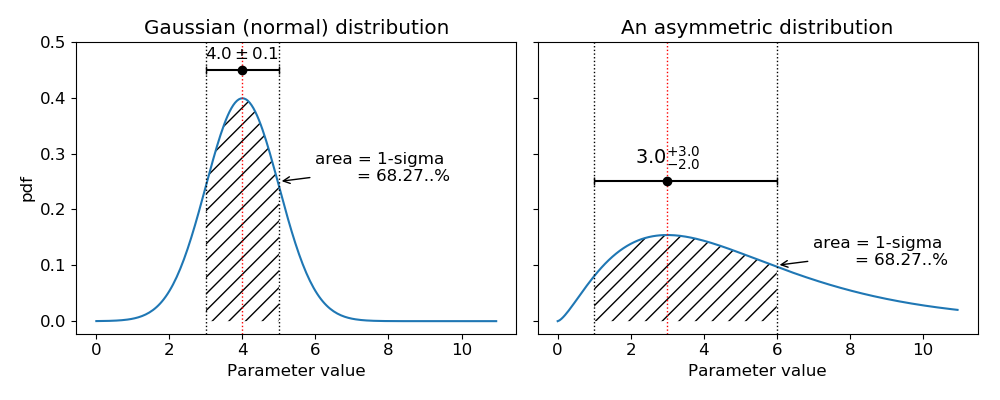
\includegraphics[width=1\linewidth]{figs/fig_posterior01}
\caption{The probability distribution function (pdf) of two examples of distributions, namely, Gaussian and an asymmetric distributions. I used a chi-square distribution for the latter for plotting purpose.}
\label{fig:figposterior01}
\end{figure}


The uncertainty ranges shown in the figure ($ 4.0 \pm 0.1 $ and $ 3.0^{+3.0}_{-2.0} $) are determined such that the lower/upper bounds include $ 68.27 \cdots \% $ of the total area. It is trivial for a Gaussian distribution: mean $ \pm $ 1-$ \sigma $. But if the distribution is asymmetric (right panel of the figure), there are few choices to set such bounds. First and the most widely used one is to set the bounds such that the distance between upper/lower bounds are minimized (but include $ 68.27 \cdots \% $ of the total area). Second is to make it symmetric while include $ 68.27 \cdots \% $ of the total area, so that you can use $ \pm $ sign for simplicity ($ 3.0 \pm 2.\mathrm{XX} $ for example). Third choice would be something like FWHM: find $ x $-axis values such that the pdf value is $ 0.5 \times \mathrm{pdf_{max}} $. The last two bounds are simple to calculate but not as accurate as the first choice.

Very assymetric probability distributions appear in cosmological sciences\footnote{Google ``posterior distribution cosmological constants''.} and exhaustive statiscal analyses are conducted on such models to reject cosmological models. The reason is that, in cosmology, we have only one single sample (our universe), and the statistical analyses given the observational data is of utmost importance. Of course similar exhaustive statistical analyses should be conducted on any research field if the data/object/target is of such importance. 



\section{Caveat on the ``$ n $-$ \sigma $ CI'' Notation}
Let me emphasize again: What we mean by ``$ n $-$ \sigma $'' is actually ``$ n $-$ \sigma $ CI'' and is \textit{not necessarily} $ n \times \sigma $. 

It maybe is tempting to convert the 1-$ \sigma $ CI to the 3-$ \sigma $ CI. For instance, from \cref{fig:figposterior01}, $ 4.0 \pm 0.1 $ and $ 3.0^{+3.0}_{-2.0} $ to $ 4.0 \pm 0.3 $ and $ 3.0^{+9.0}_{-6.0} $. This is true for the former (Gaussian) but wrong for the latter (non-Gaussian). The lower bound of the second parameter now become negative ($ 3.0 - 6.0 = -3.0 $), which is not even physically correct if this parameter is defined to be positive. What you have to do is, get the 3-$ \sigma $ CI which should contain $ 0.9973\cdots $ of the total area from the distribution given in \cref{fig:figposterior01}. There can be at least three choices to do it, which I mentioned in the previous section.


\section{Central Limit Theorem (CLT)}
The Central Limit Theorem (CLT) is at the heart of all the observational or experimental sciences. It is stated as\footnote{For strict definitions of random sample, population, independence, the statement of CLT in mathematical senses, etc, I recommend mathematical statistics textbooks.}

\begin{thm}[Central Limit Theorem; CLT] \label{thm: clt}
  Consider a random sample (observation, measurement, etc) with size $ n $ and the mean value of this sample is $ \bar{X} $. Then $ (\bar{X} - \mu) / (\sigma / \sqrt{n}) $ approaches the standard normal distribution ($ \mathcal{Z} $) as $ n \rightarrow \infty $, where $ \mu $ and $ \sigma^2 $ are the (finite) mean and variance of the population:
  \begin{equation}
    \frac{\bar{X} - \mu}{\sigma / \sqrt{n}} \sim \mathcal{Z}  \quad (\mathrm{as~} n \rightarrow \infty)~.
  \end{equation}
\end{thm}

There is one more important theorem, which we usually skip to mention:

\begin{thm}[Sample Variance Distribution] \label{thm: s and sigma}
  Consider a random sample (observation, measurement, etc) with size $ n $ and the sample variance is $ S^2 $. Then $ (n - 1) S^2 / \sigma^2 $ follows a chi-squared distribution with degrees of freedom $ (n - 1) $, where $ \sigma^2 $ is the variance of the population:
  \begin{equation}
    \frac{(n - 1) S^2}{\sigma^2 } \sim \chi^2_{(n-1)}
  \end{equation}
\end{thm}

Also the definition of the Student $ t $-distribution\footnote{This definition is directly copied from Walpole et al. p.177}:

\begin{defn}[Student $ t $-distribution]\label{def: t-distn}
  Let $ Z $ be a standard normal random variable and $ V $ a chi-squared random variable with $ v $ degrees of freedom. If $ Z $ and $ V $ are independent, then the distribution of the random variable $ T $, where
  \begin{equation}
    T = \frac{Z}{\sqrt{V /v}}
  \end{equation}
  is given by the density function
  \begin{equation}
    h(t) = \frac{\Gamma \qty[ \frac{v+1}{2} ]}{\Gamma \qty[\frac{v}{2}] \sqrt{\pi v}}
      \qty( 1 + \frac{t^2}{v} )^{-\frac{(v+1)}{2}}
    \quad ~, \quad
    -\infty < t < \infty ~.
  \end{equation}
  This is known as the Student $ t $-distribution with $ v $ degrees of freedom.
\end{defn}

We can see that the $ t $-distribution approaches the standard normal distribution as the degrees of freedom $ v \rightarrow \infty $, because the power term takes the $ e^{-t^2 / 2} $ form. 


\begin{thm}[Practical Usage of the CLT] \label{thm: practical clt}
  Consider a random sample (observation, measurement, etc) with size $ n $ large enough and the mean value of this sample is $ \bar{X} $. If $ \mu $, $ \sigma^2 $, and $ S^2 $ are the (finite) mean and variance of the population, and the sample variance, respectively:
  \begin{equation}
    \frac{\bar{X} - \mu}{S / \sqrt{{n}}} \sim T_{(n - 1)} ~.
  \end{equation}
\end{thm}

Sometimes people empirically say $ n \ge 30 $ is enough. This really depends on the situation and I will skip this issue here. The sketch of the proof of the theorem is simple. By the definition of the $ t $-distribution and Thm \ref{thm: s and sigma}, 
\begin{equation}
  T = \frac{Z}{\sqrt{V /v}} = \frac{ \frac{\bar{X} - \mu}{\sigma / \sqrt{n}} }
  {\sqrt{ \frac{(n - 1) S^2}{\sigma^2 } / (n-1)}}
  = \frac{\bar{X} - \mu}{S / \sqrt{{n}}}
\end{equation}
so the theorem is plausible. For your information, the sample variance is defined as
\begin{equation}
  S^2 := \frac{1}{n - 1} \sum_{i=1}^{n} (X - \bar{X})^2 
\end{equation}
and the sample standard deviation $ S $ is the square root of this.

Note here the difference between Thm \ref{thm: clt} and Thm \ref{thm: practical clt}: $ \sigma $ is changed to $ S $, and the standard normal distribution is changed to the $ t $-distribution of $ (n - 1) $ degrees of freedom. Since the true variance $ \sigma^2 $ is unknown, it is difficult to use the CLT (Thm \ref{thm: clt}) directly. But thanks to Thm \ref{thm: s and sigma}, we can use the variance of the sample, $ S^2 $, which is measurable, and utilize the $ t $-distribution, which is slightly bothersome than the standard normal distribution but still useful. 

Also be aware that CLT says the \textit{expectation value of the mean} is normally distributed, not the \textit{sample} is so.

\begin{ex}[Coin Tossing and the CLT]
  Consider a coin-tossing experiment and assign $ \pm 1 $ to heads and tails. Each experiment will give you $ \pm 1 $, but never $ 0 $. Meanwhile, we know a fair coin should have $ \mu = 0 $ (same probability of heads and tails). After $ n = 100 $ experiments, say you obtained $ \bar{X} = 0.01 $ and $ S = 0.1 $, so
  \begin{equation*}
    T = \frac{\bar{X} - \mu}{S / \sqrt{{n}}}
      = \frac{0.01 - \mu}{0.1 / \sqrt{100}} 
      = 1 - 100 \mu ~.
  \end{equation*}
  Since $ T \sim t_{99} $, the significance level $ \alpha = 0.05 $ confidence interval, i.e., the confidence interval containing $ 100 (1 - \alpha) \% = 95 \% $, can be
  \begin{equation*}
    t_{99, 0.025} < T < t_{99, 0.975}
    \quad \rightarrow \quad
      - 1.9842 < 1 - 100 \mu < 1.9842
    \quad \rightarrow \quad
      \mu \in [-0.0098,\, 0.0298] ~.
  \end{equation*}
  The notation $ t_{\nu, x} $ means the input argument of the $ t $-distribution with the degrees of freedom $ \nu $ such that $ \int_{-\infty}^{t_{99, x}} h(t) dt = x $. Thus, to get the two-tail CI of significance level $ \alpha $, we need to calculate $ t_{\nu, \alpha / 2} $ and $ t_{\nu, 1 - \alpha / 2} $. For a symmetric distribution like $ t $ here, $ t_{\nu, 1 - \alpha / 2} = - t_{\nu, \alpha / 2} $. This is very widely used standard notation.
  
  If you just calculated without pondering about the meaning of the caculation, you may be surprised that your next experiment gives either $ +1 $ or $ -1 $, while the expectation is $ \mu \in [-0.0098, 0.0298] $. This is because the result from CLT is, as described, about the \textit{mean} of the samples, not the \textit{single sample}. Thus, the error-bar from the CLT is not necessarily predicting the possible range of \textit{future experiments}, but it just confines the \textit{position of the mean}.
\end{ex}
The range which predicts the future experiments is called the prediction interval. You may learn the prediction interval (PI) to clarify this difference.

The two-tail significance level $ \alpha $ interval of the $ t $-distribution calculable in python by
\begin{python}
from scipy.stats import t
alpha = 0.95
nu = 99

# Note that the alpha below is NOT the significance level, 
# but the area under the curve!
lo, hi = t.interval(alpha=alpha, df=nu)
print(f"Confidence Interval: [{lo:.4f}, {hi:.4f}]")
\end{python}


\subsubsection*{Note: Uncertainty of Median}
The 1-$ \sigma $ error-bar of the median is more difficult to handle than that of the mean (CLT: Thm \ref{thm: clt}). But we can get a result from simplifying assumptions, which are not necessarily true for real observations:

\begin{thm}[Uncertainty of Median]
  Consider $ n (\gg 1) $ samples are independently drawn from $ X \sim \mathcal{G}(\mu, \sigma^2) $, a general continuous distribution with finite mean and variance $ \mu $ and $ \sigma^2 $ with pdf $ p(x) $. The uncertainty of the median estimator is 
  \begin{equation}\label{eq: err median general}
    \Delta \mathrm{med} \approx \frac{1}{2 p(\nu_0) \sqrt{n - 1}}
  \end{equation}
  and if $ \mathcal{G} =  \mathcal{N} $, i.e., a normal distribution,
  \begin{equation}\label{eq: err median}
    \Delta \mathrm{med} 
      \approx \sqrt{\frac{\pi / 2}{n - 1}} s 
      = \sqrt{\frac{\pi}{2} \frac{n}{n - 1}} \Delta \mathrm{mean}
      \approx 1.25 \Delta \mathrm{mean}
       ~,
  \end{equation}
  where $ s $ is the sample standard deviation and $ \Delta \mathrm{mean} = s / \sqrt{n} $ is the error-bar of the mean from Thm \ref{thm: practical clt}.
\end{thm}
\begin{proof}[of general distribution]
To prove it, say the true median is $ \nu_0 $ and samples $ \{ x_1, \cdots, x_n \} $ are sorted as increasing order. For an integer $ m $, set $ n = 2m + 1 $, because $ n \gg 1 $. The sample median is then $ \nu = x_{m + 1} $.
The probability of having sample median $ \nu $ is calculable by noting that we have to sample $ m $ of sample with $ x_i \le \nu $ and the other $ m $ with $ x_i > \nu $:
\begin{equation*}
  f(\nu) = \frac{n!}{m! m!} q^m (1 - q)^{m} ~,
\end{equation*}
where $ q = q(\nu) = \mathbb{P} \{ X_i \le \nu \} = \int_{-\infty}^{\nu} p(x) dx $. $ p(x) $ is the pdf of the normal distribution. 

The Taylor expansionof $ q $ at $ \nu = \nu_0 $:
\begin{equation*}
\begin{aligned}
  q(\nu) &= q(\nu_0) + \frac{1}{1!} q'(\nu_0) (\nu - \nu_0) + O\qty( (\nu - \nu_0)^2 )\\
    &\approx \frac{1}{2} + q'(\nu_0) (\nu - \nu_0) \\
    &\equiv \frac{1}{2} + p(\nu_0) (\nu - \nu_0) ~.
\end{aligned}
\end{equation*}
Then 
\begin{equation*}
\begin{aligned}
  f(\nu) &\approx \frac{n!}{m! m!}
    \qty[ \frac{1}{2} + p(\nu_0) (\nu - \nu_0) ]^m
    \qty[ \frac{1}{2} - p(\nu_0) (\nu - \nu_0) ]^m \\
    &= 
    \frac{n!}{m! m!}
    \qty[ \frac{1}{4} \qty( 1 - 4 p(\nu_0)^2 (\nu - \nu_0 )^2) ]^m \\
    &= 
    \frac{n!}{m! m! 4^m}
    \qty[ 1 - \frac{4 m p(\nu_0)^2 (\nu - \nu_0 )^2}{m} ]^m \\
    &\approx 
    \frac{n!}{m! m! 4^m}
    e^{ -4 m p(\nu_0)^2 (\nu - \nu_0 )^2 } ~.
\end{aligned}
\end{equation*}
This has the form of Gaussian distribution ($ \propto e^{-(x - \mu)^2 / 2\sigma^2} $) with mean $ \nu_0 $ and variance $ \frac{1}{4 (n-1) p(\nu_0)^2} $ since $ m = (n - 1) / 2 $. Thus, 
\begin{equation}
  \nu \sim \mathcal{N} \qty( \nu_0, \frac{1}{4 (n-1) p(\nu_0)^2} )
  \quad\rightarrow \quad
  \Delta \mathrm{med} \approx \frac{1}{2 p(\nu_0) \sqrt{n - 1}} ~.
\end{equation}
Q.E.D.
\end{proof}

\begin{proof}[of Gaussian distribution]
Now if $ p(x) $ is a Gaussian, median is equal to mean, so the pdf becomes $ p(\nu_0) = p(\mu) = \frac{1}{\sqrt{2\pi} \sigma} $, and
\begin{equation*}
  \nu \sim \mathcal{N} \qty( \nu_0, \frac{\pi / 2}{n - 1} \sigma^2 ) ~.
\end{equation*}
If we denote $ A = \sqrt{(n - 1) / (\pi / 2)} $, the statistic $ Z = A \frac{\nu - \nu_0}{\sigma} $ will follow the standard normal distribution. On the other hand, $ V = \frac{(n - 1) s^2}{\sigma^2} $ follows the chi-squared distribution of degrees of freedom $ (n - 1) $ by Thm \ref{thm: s and sigma}. Then 
\begin{equation*}
  T = \frac{Z}{\sqrt{V / (n - 1)}}
    = A \frac{\nu - \nu_0}{s}
\end{equation*}
will follow a $ t $-distribution with degrees of freedom $ (n - 1) $ by Def \ref{def: t-distn}. $ T $ is nearly a Gaussian when $ n $ is large (rule-of-thumb: when $ n \gtrsim 30 $), so 
\begin{equation}
  \nu \mathrel{\dot{\sim}} \mathcal{N} \qty( \nu_0, \frac{\pi / 2}{n - 1} s^2 )
  \quad\rightarrow \quad
  \Delta \mathrm{med} \approx \sqrt{\frac{\pi / 2}{n - 1}} s  ~.
\end{equation}
Q.E.D.
\end{proof}



\section{Meaning of the Confidence Interval}
I circunvented the definition of the CI so far. It is defined as

\begin{defn}[Confidence Interval; CI] 
  A confidence interval of significance level $ \alpha $ of a parameter $ X $ is the interval of $ X $ value such that if we conduct the identical parameter estimation process in many \textit{parallel universes} (i.e., ensemble) which have the identical true value $ X_\mathrm{true} $, fraction of $ (1 - \alpha) $ of such universes could have calculated a CI such that the $ X_\mathrm{true} $ is included in that CI.
\end{defn}

This is not a practically meaningful definition, but philosophically important. Let me give an example to elaborate the meaning of this.

\begin{ex}[Meaning of the Confidence Interval]
  Imagine there are many \textit{parallel universes} and the same observer observes the same star in each universe. Because of random errors (which we will learn later but that includes Poisson photon noise, readout noise, etc), the observer at each universe will obtain slightly different observational results. The observers will observe the star for $ n $ times, and calculate their own mean and error-bar as $ \bar{X} $ and $ S / \sqrt{n} $ from their observations. Note again that  $ S / \sqrt{n} $ is the uncertainty of the \textit{mean} value.

  For visualization, the true magnitude of the star is $ \mu = \m{14.0} $ and true standard deviation of the observation $ \sigma = \m{0.2} $ with $ n = 9 $ are used for the generation of \cref{fig:figclt01}. The universe ID 0 of both the upper and lower panels show roughly $ m = \m{14.0} \pm \m{0.1} $. That is, when the true magnitude and true standard deviation are given as $ \m{14.0} $ and $ \m{0.2} $, an observer at one of the universes (in our case universe ID 0) got $ m = \m{14.0} \pm \m{0.1} $, and that is our universe. 
\end{ex}

\begin{figure}[ht!]
  \centering
  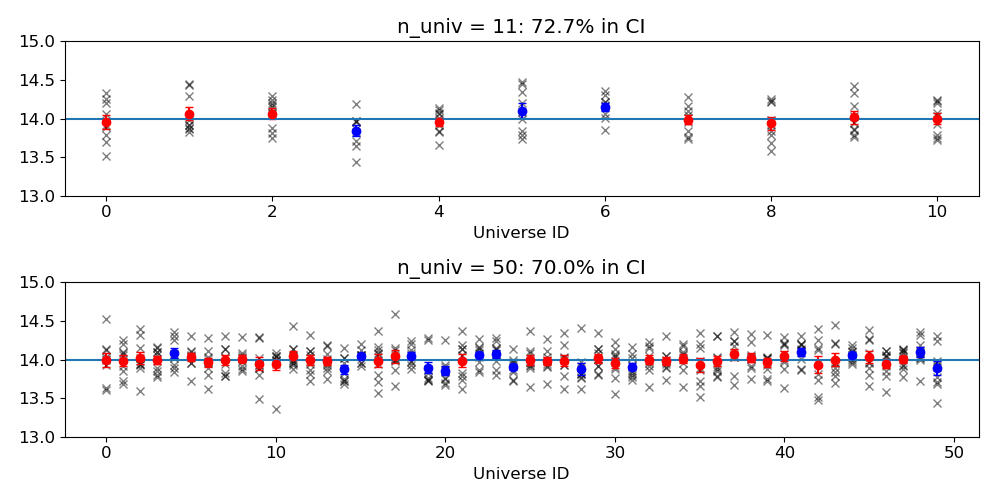
\includegraphics[width=1\linewidth]{figs/fig_clt01}
  \caption{Simulation to show the concept of CI and CLT. Black crosses are the observation in each universe, and the circles are the mean and its uncertainty from the CLT $ S / \sqrt{n} $. Red circles are the univserses where the confidence interval contains the true mean $ \mu = \m{14.0} $ and blue circles are the others. In the title, the fraction of the universes which contains the true mean within their own confidence intervals out of \texttt{n\_univ} simulated universes is shown. This fraction approaches $ 0.6827\cdots $ as the number of universe gets infinity.}
  \label{fig:figclt01}
\end{figure}

I will close this section with an excerpt from Walpole p.234:

\textit{The interpretation of a CI is often misunderstood. It is tempting to conclude that the parameter falls inside the CI with probability of(, e.g.,) 0.95. (But this is not ture.) A CI merely suggests that if the experiment is conducted and data are observed again and again, about 95\% of such intervals will contain the true parameter.}



\section{Answer to the Question}
In statistics, the \textit{null hypothesis}, denoted $ H_0 $, is the one that is the simplest, and that has value if it is \textit{rejected} (not \textit{accepted}). The \textit{alternative hypothesis}, $ H_1 $, is another possibility if $ H_0 $ is not true. In the simplest case, $ H_1 $ is the complementary of $ H_0 $. For example, $ H_0: \mu = 0 $ and $ H_1: \mu \neq 0 $. 

Let's consider the opening question: $ m = \m{14.0} \pm \m{0.1} $. Now you understand that $ \m{14.0} $ means that the mean value\footnote{It can actually be the median value, most probable value, or whatever the representative value.} from the observation, and $ \pm \m{0.1} $ means the uncertainty or the error-bar of the Gaussian probability distribution of that mean value, $ S / \sqrt{n} $. If it were not Gaussian, the author should have given more information. Note that the sample standard deviation is $ \sqrt{n} $ times the error-bar.

To answer the question, we set the hypotheses\footnote{There are some ``standard'' ways to set the hypotheses, and it may seem very sudden if you are not familiar with these. Please refer to basic applied statistics textbooks for more examples, e.g., p.246 and p.264 of Walpole et al.}:
\begin{equation}
  H_0 : m_1 = m_2 
  \sep
  H_1 : m_1 \neq m_2 ~,
\end{equation}
where $ m_1 = \m{14.0} \pm \m{0.1} $ and $ m_2 $ is the other (from researcher 2). $ m_1 $ and $ m_2 $ here means the ``true'' magnitude of the star, not the measured value! If it were the measured value, they are just different, since one is 14.0 and the other is 15.0. The two true means may be different because (1) researchers may have mistakenly observed different star, (2) the star is maybe a variable (including binary), (3) explanet occulted some part of the star, or any other scenario is possible.

Now we have to choose which formula to use. When two measurements with $ \bar{x}_1 \pm s_1 $ and $ \bar{x}_2 \pm s_2 $ from the number of observations $ n_1 $ and $ n_2 $ are given, and $ \mu_1 $ and $ \mu_2 $ are the true means of two sampling distributions that will be tested under the hypothesis testing, there are two different formulae:
\begin{itemize}
\item The true variances are unknown and different (Satterthwhite approximation\footnote{SatterthwhiteFE (1946, Biometrics Bulletin, 2, 110), ``An Approximate Distribution of Estimates of Variance Components.''}):
\begin{equation}
  t = \frac{(\bar{x}_1 - \bar{x}_2) - (\mu_1 - \mu_2) }{\sqrt{s_1^2 / n_1 + s_2^2 / n_2}}
\end{equation}
follows the $ t $-distribution with degrees of freedom
\begin{equation}
  \nu \approx 
    \frac{\qty( s_1^2 / n_1 + s_2^2 / n_2 )^2}
    {\frac{ \qty(s_1^2 / n_1)^2 }{n_1 - 1}
      + \frac{ \qty(s_2^2 / n_2)^2 }{n_2 - 1}} ~.
\end{equation}
\item The true variances are unknown but the same:
\begin{equation}
  t = \frac{(\bar{x}_1 - \bar{x}_2) - (\mu_1 - \mu_2) }{s_p \sqrt{1 / n_1 + 1 / n_2}}
\end{equation}
follows the $ t $-distribution with degrees of freedom $ \nu = n_1 + n_2 - 2 $ and
\begin{equation}
  s_p = \frac{(n_1 - 1) s_1^2 + (n_2 - 1) s_2^2}{\nu} ~.
\end{equation}
\end{itemize}
Which one will you choose? To answer our original question, it is more reasonable to assume the true variances are not necessarily identical, because they may have used different instruments at different sky conditions. So I will use the first choice.

To apply the formula, you need the number of observations from each researcher, i.e., the $ n_1 $ and $ n_2 $ values. As I mentioned, it is an ill-defined question since this numbers are not given. So let me assume $ n_1 = n_2 = n = 5 $. The question can be reformulated as $ \bar{x}_1 = 14.0 $, $ \bar{x}_2 = 15.0 $, $ s_1 = 0.1 \sqrt{n} $, and $ s_2 = 1.0\sqrt{n},\, 0.3\sqrt{n}, \, 0.1\sqrt{n} $, where I dropped the magnitude sign for brevity. Under the null hypothesis ($ H_0: \mu_1 = \mu_2 $), $ \mu_1 - \mu_2 = 0 $. For the three $ s_2 $ values, 
\begin{equation}
\begin{aligned}
  t &= \frac{(14.0 - 15.0) - 0}{\sqrt{(s_1^2 + s_2^2) / n}}
  \quad &&\rightarrow \quad
  t &&= & -0.995 ,\, && -3.162 ,\, && -7.07 \\
  \nu &= (s_1^2 + s_2^2) (n-1)
  \quad &&\rightarrow \quad
  \nu &&= & 4.08, \, && 4.32, \, && 8.0 \\
  &&&&&\approx & 4 ,\, && 4 ,\, && 8 \\
\end{aligned}
\end{equation}
The values are in the order for $ s_2 = (1.0,\, 0.3, \, 0.1)\sqrt{n} $ cases. The (two-tail) significance level $ \alpha $ test is listed in \cref{tab: CI}.

\begin{table}[ht!]
\centering
\caption{The confidence interval calculation for the example question.}
\label{tab: CI}
\begin{tabular}{c|c||c|c}
CI \% & significance level $ \alpha $ and $ \frac{\alpha}{2} $& $ \nu = 4 $ case & $ \nu = 8 $ case \\
\hline
90 \% & 0.10 \& 0.05   & $ [-2.1318, 2.1318] $ & $ [-1.8595, 1.8595] $ \\
95 \% & 0.05 \& 0.025  & $ [-2.7764, 2.7764] $ & $ [-2.3060, 2.3060] $ \\
99 \% & 0.01 \& 0.005  & $ [-4.6041, 4.6041] $ & $ [-3.3554, 3.3554] $ \\
\end{tabular}
\end{table}

The answers to the questions are, assuming $ n_1 = n_2 = 5 $,
\begin{itemize}
\item Case A ($ t = -0.995 $ with $ \nu = 4 $): The $ t $ value is inside of all three CIs. Thus, we cannot reject $ H_0 $ under 90 \%, 95 \%, and 99 \% CI criterion (cannot reject under the significance level $ \alpha = 0.10,\, 0.05,\, 0.01 $).
\item Case B ($ t = -3.162 $ with $ \nu = 4 $): The $ t $ value is inside of 90 \% and 95 \% CI but outside of the 99 \% CI. Thus, we reject $ H_0 $ with $ \alpha = 0.10 $ and $ 0.05 $, but cannot reject it with $ \alpha = 0.01 $.
\item Case C ($ t = -7.07 $ with $ \nu = 8 $): We reject $ H_0 $ with all the three $ \alpha = 0.10,\, 0.05,\, 0.01 $.
\end{itemize}
\vspace{\parskip}

By \textit{rejecting the null hypothesis}, $ H_0: m_1 = m_2 $, we mean that it is unlikely that the true magnitude value of the two studies are identical. By \textit{failing in rejecting the null hypothesis}, we mean that it is impossible to conclude whether $ m_1 $ and $ m_2 $ are the same under the given significance level. 

The results are as expected: For Case A, the error-bar of $ m_2 $ is too large, which means it is almost impossible to reject the claim that $ m_1 = m_2 $, so the we always fail to reject the null hypothesis. For Case C, the error-bars are too small and thus $ m_1 $ is of course vastly different from $ m_2 $, so the null hypothesis is always rejected.

%\footnote{You may wonder what if we have $ n = 1 $. The $ \nu $ is undetermined and all the calculation seem to meaningless, but of course we can have error-bars for each single observation. That is not considered in this example since here we are simply assuming the mean is inferred from $ n $ observations under the CLT, and we need $ n > 1 $ to calculate the sample variance $ S^2 $. I will not consider the error-bars of each observations. Such a detailed statistical analyses should follow some well-developed and specific statistical routines available in your research field.}.
%In this example we do not care about the error-bar of each observation but the final error-bar of the mean value from researchers. If we want to consider the error-bars of every observations, this kind of classical statistical method gets very complicated and almost impossible to give meaningful results. You then need Bayesian approach and Monte Carlo simulation technique.




\section{Poisson Noise}
The Poisson process is a fancy naming for some special ``counting''. In astronomy, we count photons (well, actually the CCD counts the electrons) over time, in social sciences we can count the death toll over time, in experiments we could count the lattice of a randomly shaped crystal over the distance. A formal definition is\footnote{See, e.g., \url{http://dept.stat.lsa.umich.edu/~ionides/620/notes/poisson_processes.pdf} and \url{https://www.probabilitycourse.com/chapter11/11_1_2_basic_concepts_of_the_poisson_process.php}}

\begin{defn}[Poisson Process 1]
The Poisson process $ N(t) $ for $ t \ge 0 $ ($ t $ can be time, distance, or similar things), with rate $ \lambda $ is defined by
\begin{enumerate}
\item $ N(0) = 0 $
\item $ N(t) $ has independent increment
\item $ N(t_2) - N(t_1) $ follows Poisson distribution of rate $ \lambda (t_2 - t_1) $ for $ t_1 < t_2 $.
\end{enumerate}
\end{defn}

It can be proven that it is identical to 

\begin{defn}[Poisson Process 2]
The Poisson process $ N(t) $ for $ t \ge 0 $ ($ t $ can be time, distance, or similar things), with rate $ \lambda $ is defined by
\begin{enumerate}
\item $ N(0) = 0 $
\item $ N(t) $ has independent increment
\item $ \mathbb{P}(N(h) = 1) = \lambda h + o(h) $ for small $ h $.
\item $ \mathbb{P}(N(h) \ge 2) = o(h) $ for small $ h $.
\end{enumerate}
\end{defn}

Here $ o(h) $ is any function such that $ \lim_{h \rightarrow 0} o(h) / h = 0 $. The last two items in this second definition can be re-phrased like this:
\begin{itemize}
\item [3.] For a very small interval $ h $, the probability of one single ``counting'' (Poisson process) occurs in that interval is proportional to the length of $ h $.
\item [4.] For a very small interval $ h $, the probability of two or more ``counting'' (Poisson process) occurs in that interval is nearly 0.
\end{itemize}
These must be independent of whether the counting happened outside of the interval, because the second item of the definition states the increment is independent.
\newpage
\begin{ex}[Photon Counting and Poisson Process]
The photon counting process of astronomy resembles the Poisson Process. If $ N(t) $ is the number of photons or electrons under the exposure time $ t $, it is trivial that the first two items of the definition is satisfied. Next, use the rephrased version of the next items. The number of photons hitting CCD with infinitesimal time interval $ h = dt $ must be 0 or 1, but not larger than 1 (e.g., if a pixel count is 10,000 after 10 sec of exposure, we can take $ h \ll \SI{10}{s} / 10,000 = \SI{1}{ms} $ to meet this condition). Thus, photon counting is a Poisson process.
\end{ex}

The Poisson process follow the Poisson distribution:

\begin{defn}[Poisson Distribution] \label{def: Pois pdf}
The Poisson process of rate $ \lambda $ has the following pdf
\begin{equation} \label{eq: Pois pdf}
  p(x; \lambda t) = \frac{(\lambda t)^{x}}{x!} e^{-\lambda t}
\end{equation}
for non-negative integer $ x $.
\end{defn}

\begin{thm}[Poisson Distribution Mean and Variance] \label{thm: Pois mean std}
The mean, variance, and the standard deviation of the Poisson distribution $ p(x; \lambda t) $ are
\begin{equation}\label{eq: Pois mean std}
  \mathrm{mean} = \lambda t
  \sep
  \mathrm{var} = \lambda t
  \sep
  \mathrm{std} = \sqrt{\lambda t} ~.
\end{equation}
\end{thm}
The reason we use $ \lambda t $ not just $ \lambda $ is clear from Thm \ref{thm: Pois mean std}: the mean changes as $ t $ changes, and we want to express $ p(x; \mathrm{mean}) $ rather than $ p(x; \mathrm{mean} / t) $. For instance, if the photon influx is $ \lambda = \SI{10}{photons / s} $, the mean of photon count is a function of time as $ \lambda t $, so for $ t = \SI{10}{s} $, the pdf is $ p(x; \SI{100}{photons}) $. If the particles are distributed with mean density along the line of sight $ \lambda = \SI{0.1}{particle / m} $, the mean of particles along the line of sight is a function of the reaching distance $ \lambda d $, so the pdf for $ d = \SI{5}{m} $ is $ p(x; \SI{0.5}{particles}) $. 

\begin{thm}[Poisson to Gaussian] \label{thm: Pois gauss}
As $ x \rightarrow \infty $, the Poisson distribution approaches normal distribution $ \mathcal{N}( \lambda t, \lambda t ) $.
\end{thm}
Although I will omit here, the proof uses Stirling's formula $ x! \approx \sqrt{2\pi x} x^x e^{-x} $ and $ \ln[ (1 + \varepsilon)^{\lambda t (1 + \varepsilon) + 1 / 2 }] \approx \lambda t \varepsilon + \lambda t \varepsilon^2 / 2 $, where $ x = \lambda t ( 1 + \varepsilon ) $ with $ \lambda t \gg 1 $ and $ \varepsilon \ll 1 $. Stirling's formula has relative error of less than 1 \% when $ x = 1 $ and is almost negligible for any $ x $ of interest in many cases. Considering all the approximations in the proof, we can safely assume that Poisson distribution is quite Gaussian (normal) in many astronomical contexts, unless $ x $ is very small ($ \lesssim 10 $..?).

\begin{ex}[Photon Counting and Poisson Noise]
We saw the photon or electron counting is a Poisson process. Thus, we can use \cref{eq: Pois pdf,eq: Pois mean std}. For example, if we collected 10,000 electrons, the 1-$ \sigma $ uncertainty (1-$ \sigma $ CI) or the standard deviation of this counting is $ \sqrt{10,000} = 100 $, so we denote $ N = 10,000 \pm 100 $. Since the $ N $ is large enough, Thm \ref{thm: Pois gauss} says this is just a Gaussian distribution of mean 10,000 and standard deviation 100 (1 \% of the mean). Since magnitude is $ (\mathrm{const}) - 2.5 \lg (\mathrm{count}) $, differentiation gives a first-order estimation of the uncertainty in the magnitude $ \Delta m = -\frac{2.5}{\ln 10} \frac{\Delta (\mathrm{count})}{\mathrm{count}} = \m{0.01} $ (error-bar), which is small enough for some scientific purposes.
\end{ex}

The next example is not directly related to Poisson process, but related to the binomial distribution (Bernoulli process) which has the pdf of $ b(x; n, p) = \binom{n}{x} p^x (1 - p)^{n - x} $ for getting $ x $ outcomes from $ n $ trials with $ p $ probability to have outcome. The pdf of binomial process approaches Poisson pdf with $ p(x; np) $ when $ n \rightarrow \infty $, $ p \rightarrow 0 $ but $ np $ is finite. Thus, the mean, variance, and standard deviation of such binomial distribution is calculabe using Thm \ref{thm: Pois mean std}.
\begin{ex}[Babies in Hospital: Provided by Prof. Jae-Kwang Kim at KAIST]
There are two hospitals A and B. New babies are born as either sex chromosome XX/XY with probability 50:50. Everyday A gives birth to 45 babies and B to 15 babies. Each hospital recorded the number of days when more than 60 \% of babies are girl.
\begin{enumerate}
\item Which hospital will have more such days?
\item With how much confidence can you say so?
\end{enumerate}
\end{ex}


\section{Error Propagation}
When we have to calculate the uncertainty of a parameter derived from other parameters that have their own uncertainties, what we usually use is the \textit{error propagation}. For example, $ \mathrm{g'} = 14.0 \pm 0.1 $ and $ \mathrm{r'} = 15.0 \pm 0.1 $, what is the uncertainty of the $ \mathrm{g' - r'} $ color? Many astronomers will say it is $ -1.0 \pm 0.14 $, where the error here is $ \sqrt{\sigma_\mathrm{g'}^2 + \sigma_\mathrm{r'}^2} $ ($ \sigma $ is the error-bar). If the temperature is $ T = 100 \pm 1 \si{K} $, what is the fractional uncertainty of bolometric luminosity ($ L = \sigma_\mathrm{SB} T^4 $)? Now people will say $ \Delta L / L \approx \frac{4 \sigma_\mathrm{SB} T^3 \Delta T }{\sigma_\mathrm{SB} T^4} = 4 \Delta T / T = 4 \% $. 

The way how we do this is that, for a function $ f = f(x| a, b, c) $ where $ (a, b, c) $ is a set of parameters:
\begin{equation}\label{eq: error propagation}
  (\Delta f)^2 \approx 
    \qty(\frac{\partial f}{\partial a} \Delta a)^2
    + \qty(\frac{\partial f}{\partial b} \Delta b)^2
    + \qty(\frac{\partial f}{\partial c} \Delta c)^2
\end{equation}
If any parameters are dependent, we need a covariance term $ \sigma_{ab} $ for instance, and this is one of the reasons why the above error-propagation is only an approximation. This formual itself is similar to getting the gradient. 

Note that this is only an approximation, and in reality, we need more complicated calculation. Note that it is impossible to know how accurate this approximation is, before you conduct detailed calculation. The reason astronomers use it in spite of the pitfall is because most cases we are only interested in the rough estimation of the error-bar.




\section{The Chi-Square Minimization}
You may have heard of it, or simply the \textit{least square} something. Least square or the chi-square minimization is a process to find the set(s) of model parameters which has the biggest (or bigger than threshold) \textit{likelihood} in Bayesian statistics. The set of ``best'' model parameters is the one with the largest likelihood, so we call it the maximum likelihood estimator, \textbf{MLE}.

Consider independent and identically distributed (\textit{i.i.d.}) random variables\footnote{Random variables $ X_{i} $ for $ i = 0, \cdots, N $ are called i.i.d. if they (1) follow identical probability distribution, say $ f(x) $, and (2) $ f(X = x) = f(X_1 = x_1) \times \cdots \times f(X_N = x_N) $, where $ x = (x_1, \cdots , x_N) $ (same for $ X $). }, e.g., flux as a function of $ \lambda $. It is independent because the measurement at each wavelength itself is independent from that of any other wavelength. It is identically distributed because and we will assume each error-bar is Gaussian. The second assumption is not necessarily correct, and actually that happens many times (e.g., flux is Gaussian distributed but magnitude is not, because it is log of Gaussian distribution).

The Bayes' theorem will be studeid in later, but let me introduce it first to grap the meaning of chi-square statistic:
\begin{align*}
  P(\mathbf{\theta}|D, I) &= \frac{P(D|\mathbf{\theta}, I) P(\mathbf{\theta}|I)}{P(D, I)} \\
  P(\theta|D, I) &\propto P(D | \theta, I) P(\theta|I)
\end{align*}
When we have data points, $ (x_i, y_i) $, which are all independent, and $ y \sim N(y_i, \sigma_i^2) $. Then one of the most na\"{i}ve goodness-of-fit statistic variables can be the square-sumed error:
\begin{equation}\label{eq: sse}
  \mathrm{SSE} = \sum_{i} (y_i - f(x_i| \theta))^2
\end{equation}
Since $ y_i $ are all Gaussian, the probability of obtaining such data is obtained from the multiplication law:
\begin{equation*}
  P(D = \{y_i\}) = \Pi_i A e^{-(f(x_i|\theta)-y_i)^2/2\sigma_i^2} 
\end{equation*}
or taking log:
\begin{equation}
  \ln P(D = \{y_i\}) = \ln A \sum_i -(f(x_i|\theta)-y_i)^2/2\sigma_i^2
\end{equation}
Now getting parameters which maximize $ P $ is identical to (1) getting them which maximize $ \ln P $, and this is also identical to (2) getting them which mininize the summation in the exponent. Therefore, the exponent is defined as the chi-square statistic as:
\begin{equation}\label{eq: chi-square statistic}
  \chi^2 = \sum_i \frac{(y_i - f(x_i | \theta))^2}{\sigma_i^2}
\end{equation}




\section{Interpolation}
When we fit an analytic function to the data, we usually use a statistic (e.g., the chi-square value or the BIC) that indicates the goodness-of-fit (also called figure of merit). But what if we don't know or not interested in the true analytic function behind the scene? For example, for aperture trace or sense function in spectroscopy, we have absolutely no idea what is the true analytic function. In this situation, \textbf{interpolation} comes in. 

\begin{defn}[Interpolation]
An interpolation function is a function that smoothly connects \textit{all} the observed data points.
\end{defn}

For instance, a linear interpolation is a function which connects all the data points with linear segments as in \cref{fig:interpolation}. In cubic spline, you fit a 3rd order polynomial function (total 4 unknowns). For points $ (x_i, y_i) $ where $ i = 0 \ldots n $, we want to obtain $ n $ spline curves $ S_i(x) $ for $ i = 0 \ldots n-1 $. All such interpolation functions should be \textit{smoothly connected} to each other by
\begin{itemize}
  \item $ S_i (x_i ) = y_i      \quad(i = 0 , \ldots , n-1). $
  \item $ S_{i-1} (x_i ) = y_i  \quad(i = 1 , \ldots , n). $
  \item $ S^\prime_i (x_i) = S^\prime_{i-1} (x_i)\quad(i = 1 , \ldots , n-1). $
  \item $ S^{\prime\prime}_i (x_i) = S^{\prime\prime}_{i-1} (x_i) \quad(i = 1 , \ldots , n-1). $
  \item $ S^{\prime\prime}_0 (x_0) = S^{\prime\prime}_{n-1} (x_n) =0 $.
\end{itemize}

\begin{figure}
  \centering
  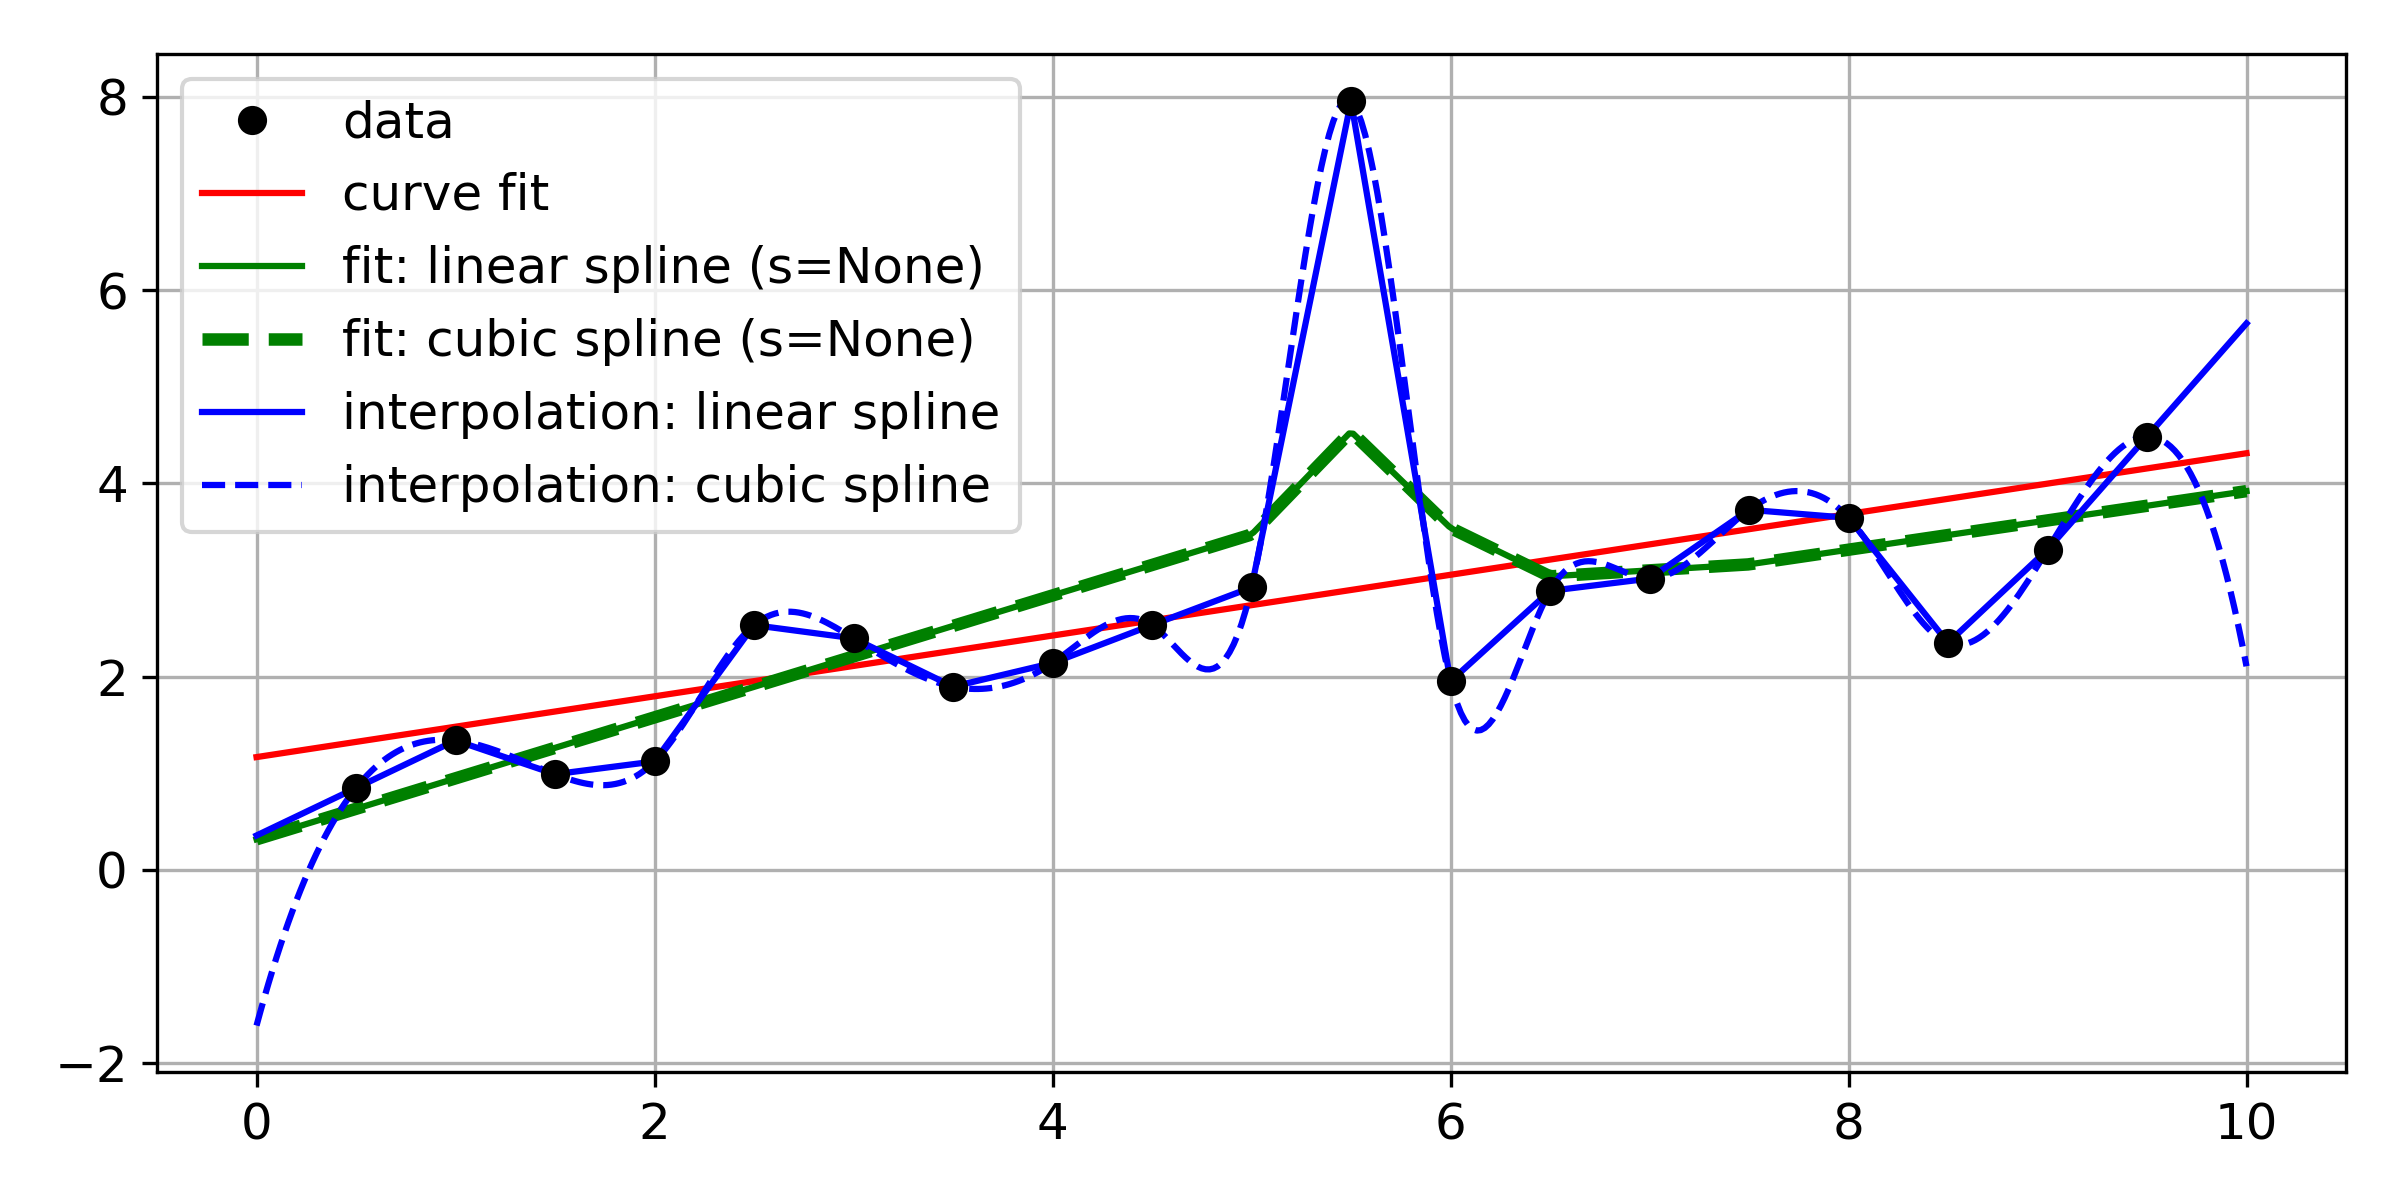
\includegraphics[width=0.7\linewidth]{figs/interpolation}
  \caption{A display of linear/cubic spline interpolations and spline fittings.}
  \label{fig:interpolation}
\end{figure}

In python, you can use
\begin{python}
from scipy.interpolate import UnivariateSpline
# linear spline interpolation
interp_1 = UnivariateSpline(x, y, s=0, k=1)
# cubic spline interpolation
interp_3 = UnivariateSpline(x, y, s=0, k=3)

# use it as y_interp_1 = interp_1(x_values)
\end{python}
The parameter \texttt{s} is the smoothing factor. That is, 
\begin{equation}
  \sum_{i=1}^{n} w_i^2 (y_i - S(x_i))^2 \le s ~.
\end{equation}
If no error-bar is present, we can just ignore $ w_i $ (weights), and if there exists $ \sigma_i $, we can use $ w_i = 1/\sigma_i $, and the above equation becomes nothing but a chi-square. In that case, the $ \chi^2 $ smaller than the total degrees of freedom (roughly the number of data points) is a good measure, so \pyth{s = len(x)} is a good guess for spline fitting. If you put $ s = 0 $, it means $ S(x_i) $ must be the same as $ y_i $, i.e., the fitted function must go through all the data points: this is the interpolation. 

From the figure, cubic spline interpolation is more smooth and the linear one looks too discrete, so you may always want to use cubic version. A caveat is that cubic spline has large fluctuation when there is any large scatter, as seen from $ x = 5 $ and $ x = 6 $. This ``shooting'' effect is severe when you fit a sense function (spectroscopic flux calibration) to a spectroscopic standard star: if the star has an absorption line, the cubic fit will be problematic near that wavelength region. 
